\chapter{Geometrija v ravnini}

\section{Osnovni geometrijski pojmi}

            
                Evklid je v prvi knjigi \textit{Elementov} postavil $23$ 'opredelitev' temeljnih geometrijskih pojmov.
                Med njimi so:
                \begin{itemize}
                    \item \textbf{Točka} je tisto, kar nima delov -- nima razsežnosti.
                    \item \textbf{Črta} je dolžina brez širine -- ena razsežnost.
                    \item \textbf{Ploskev} je tisto, kar ima samo dolžino in širino -- dve razsežnosti.
                \end{itemize}
            
                ~
            
                Tem trditvam sledijo \textbf{aksiomi} (temeljne resnice) -- privzamemo jih kot veljavne hipoteze,
                 \textbf{izreki}~-- dokazujemo jih z aksiomi in prej dokazanimi izreki, 
                 in \textbf{definicije} -- opisi novih pojmov in lastnosti.
            
        
                ~
        
            \subsection*{Incidenčni aksiomi}

            \begin{definicija}
                \textit{Incidenca} je relacija, ki povezuje točko in premico -- premica in točka sta v relaciji,
                 če točka leži na premici; $A~R~p$, če $A\in p$.
            \end{definicija}

            \begin{aksiom}
                Za dve različni točki $A$ in $B$ obstaja natanko določena premica $p$, tako da točki $A$ in $B$ ležita na njej.
            \end{aksiom}

            \begin{aksiom}
                Za vsako premico $p$ obstajata vsaj dve različni točki $P$ in $Q$, ki ležita na njej.
            \end{aksiom}

            \begin{aksiom}
                Obstajajo tri različne točke, ki ne ležijo hkrati na isti premici.
            \end{aksiom}
        

            ~
        
            \begin{definicija}
                Točke $A_1, A_2, A_3, \dots$, ki ležijo na isti premici, so \textbf{kolinearne}, 
                če ne ležijo na isti premici, pa so \textbf{nekolinearne}.
            \end{definicija}

            ~

            \begin{izrek}
                Dve različni premici imata lahko največ eno skupno točko.
            \end{izrek}

            \begin{definicija}
                Premici, ki imata natanko eno skupno točko, se \textbf{sekata}, imenujemo ju \textbf{sečnici},
                njuno skupno točko pa \textbf{presečišče} premic.
            \end{definicija}

            \begin{definicija}
                Premici, ki ležita na isti ravnini in nimata nobene skupne točke ali imata vse točke skupne -- sovpadata, sta \textbf{vzporedni}, imenujemo ju \textbf{vzporednici}.
            \end{definicija}
        

            ~
        
            \begin{aksiom}
                Če so tri različne točke kolinearne, ena vedno leži med drugima dvema.

                \begin{figure}[H]
                    \centering
                    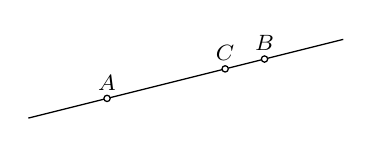
\begin{tikzpicture}
                        % \clip (0,0) rectangle (14.000000,10.000000);
                        {\footnotesize

                        % Drawing line A B
                        \draw [line width=0.016cm] (1.000000,1.250000) -- (1.961194,1.490299);%
                        \draw [line width=0.016cm] (2.038806,1.509701) -- (3.461194,1.865299);%
                        \draw [line width=0.016cm] (3.538806,1.884701) -- (3.961194,1.990299);%
                        \draw [line width=0.016cm] (4.038806,2.009701) -- (5.000000,2.250000);%

                        % Marking point A by circle
                        \draw [line width=0.016cm] (2.000000,1.500000) circle (0.040000);%
                        \draw (2.000000,1.500000) node [anchor=south] { $A$ };%

                        % Marking point C by circle
                        \draw [line width=0.016cm] (3.500000,1.875000) circle (0.040000);%
                        \draw (3.500000,1.875000) node [anchor=south] { $C$ };%

                        % Marking point B by circle
                        \draw [line width=0.016cm] (4.000000,2.000000) circle (0.040000);%
                        \draw (4.000000,2.000000) node [anchor=south] { $B$ };%
                        }
                    \end{tikzpicture}
                \end{figure}
            \end{aksiom}

            \begin{aksiom}
                Če sta $A$ in $B$ različni točki premice $p$, potem na premici $p$ ležita vsaj še točki $C$ in $D$,
                in sicer $C$ leži med $A$ in $B$, $D$ pa tako, da je $C$ med $A$ in $D$.

                \begin{figure}[H]
                    \centering
                    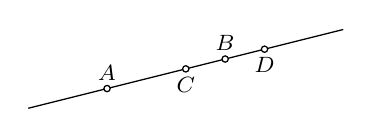
\begin{tikzpicture}
                        % \clip (0,0) rectangle (14.000000,10.000000);
                        {\footnotesize

                        % Drawing line A B
                        \draw [line width=0.016cm] (1.000000,1.250000) -- (1.961194,1.490299);%
                        \draw [line width=0.016cm] (2.038806,1.509701) -- (2.961194,1.740299);%
                        \draw [line width=0.016cm] (3.038806,1.759701) -- (3.461194,1.865299);%
                        \draw [line width=0.016cm] (3.538806,1.884701) -- (3.961194,1.990299);%
                        \draw [line width=0.016cm] (4.038806,2.009701) -- (5.000000,2.250000);%

                        % Marking point A by circle
                        \draw [line width=0.016cm] (2.000000,1.500000) circle (0.040000);%
                        \draw (2.000000,1.500000) node [anchor=south] { $A$ };%

                        % Marking point C by circle
                        \draw [line width=0.016cm] (3.000000,1.750000) circle (0.040000);%
                        \draw (3.000000,1.750000) node [anchor=north] { $C$ };%

                        % Marking point B by circle
                        \draw [line width=0.016cm] (3.500000,1.875000) circle (0.040000);%
                        \draw (3.500000,1.875000) node [anchor=south] { $B$ };%

                        % Marking point D by circle
                        \draw [line width=0.016cm] (4.000000,2.000000) circle (0.040000);%
                        \draw (4.000000,2.000000) node [anchor=north] { $D$ };%
                        }
                    \end{tikzpicture}
                \end{figure}
            \end{aksiom}

            \begin{izrek}
                Med dvema različnima točkama premice je neskončno mnogo točk.
            \end{izrek}

        
            ~

        
            \begin{definicija}
                Množica točk premice, ki ležijo med različnima točkama $A$ in $B$, vključno z $A$ in $B$,
                je \textbf{daljica~$AB$}. Točki $A$ in $B$ sta njeni \textbf{krajišči}.

                \begin{figure}[H]
                    \centering
                    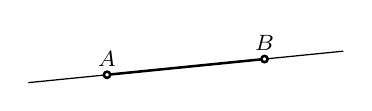
\begin{tikzpicture}
                        % \clip (0,0) rectangle (14.000000,10.000000);
                        {\footnotesize

                        % Drawing line A B
                        \draw [line width=0.016cm] (1.000000,1.400000) -- (1.960199,1.496020);%
                        \draw [line width=0.016cm] (2.039801,1.503980) -- (3.960199,1.696020);%
                        \draw [line width=0.016cm] (4.039801,1.703980) -- (5.000000,1.800000);%

                        % Drawing segment A B
                        \draw [line width=0.032cm] (2.039801,1.503980) -- (3.960199,1.696020);%

                        % Marking point A by circle
                        \draw [line width=0.032cm] (2.000000,1.500000) circle (0.040000);%
                        \draw (2.000000,1.500000) node [anchor=south] { $A$ };%

                        % Marking point B by circle
                        \draw [line width=0.032cm] (4.000000,1.700000) circle (0.040000);%
                        \draw (4.000000,1.700000) node [anchor=south] { $B$ };%
                        }
                    \end{tikzpicture}
                \end{figure}
            \end{definicija}

            \begin{definicija}
                Poljubna točka premice razdeli premico na dva \textbf{poltraka}. To točko imenujemo \textbf{izhodišče}, ponavadi jo označimo z $O$.

                \begin{figure}[H]
                    \centering
                    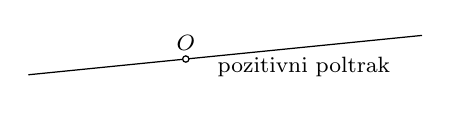
\begin{tikzpicture}
                        % \clip (0,0) rectangle (14.000000,10.000000);
                        {\footnotesize

                        % Drawing line O B
                        \draw [line width=0.016cm] (1.000000,1.300000) -- (2.960199,1.496020);%
                        \draw [line width=0.016cm] (3.039801,1.503980) -- (6.000000,1.800000);%

                        % Marking point O by circle
                        \draw [line width=0.016cm] (3.000000,1.500000) circle (0.040000);%
                        \draw (3.000000,1.500000) node [anchor=south] { $O$ };%

                        % Marking point poz
                        \draw (4.500000,1.400000) node  {pozitivni poltrak };%
                        }
                    \end{tikzpicture}
                \end{figure}
            \end{definicija}

            \begin{definicija}
                Premica, na kateri leži daljica oziroma poltrak, je \textbf{nosilka} daljice oziroma poltraka.
            \end{definicija}
        

            ~
        
            \begin{definicija}
                \textbf{Enostavni lik} je množica točk v ravnini, ki jo omejuje sklenjena krivulja, ki sama sebe ne seka.
            \end{definicija}

            \begin{definicija}

                Množica točk v ravnini je \textbf{konveksna}, če za poljubni točki $A$ in $B$ iz te množice velja, da je daljica $AB$ njena podmnožica.
                
                \begin{multicols}{2}
                $$ \mathcal{M}\text{~konveksna} \Leftrightarrow \forall A, B\in\mathcal{M}\Rightarrow AB\subseteq\mathcal{M} $$
                ~\\~

                \begin{figure}[H]
                    \centering
                    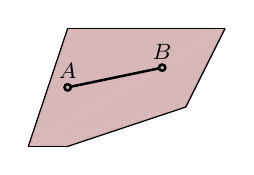
\begin{tikzpicture}
                        % \clip (0,0) rectangle (14.000000,10.000000);
                        {\footnotesize

                        % Changing color 215 183 183
                        \definecolor{r215g183b183}{rgb}{0.843137,0.717647,0.717647}%
                        \color{r215g183b183}% 

                        % Filling triangle C D E
                        \fill (1.500000,1.500000) -- (2.000000,1.500000) -- (3.500000,2.000000);%

                        % Filling triangle C E F
                        \fill (1.500000,1.500000) -- (3.500000,2.000000) -- (4.000000,3.000000);%

                        % Filling triangle C F G
                        \fill (1.500000,1.500000) -- (4.000000,3.000000) -- (2.000000,3.000000);%

                        % Changing color 0 0 0
                        \definecolor{r0g0b0}{rgb}{0.000000,0.000000,0.000000}%
                        \color{r0g0b0}% 

                        % Drawing segment C D
                        \draw [line width=0.016cm] (1.500000,1.500000) -- (2.000000,1.500000);%

                        % Drawing segment D E
                        \draw [line width=0.016cm] (2.000000,1.500000) -- (3.500000,2.000000);%

                        % Drawing segment E F
                        \draw [line width=0.016cm] (3.500000,2.000000) -- (4.000000,3.000000);%

                        % Drawing segment F G
                        \draw [line width=0.016cm] (4.000000,3.000000) -- (2.000000,3.000000);%

                        % Drawing segment G C
                        \draw [line width=0.016cm] (2.000000,3.000000) -- (1.500000,1.500000);%

                        % Marking point A by circle
                        \draw [line width=0.032cm] (2.000000,2.250000) circle (0.040000);%
                        \draw (2.000000,2.250000) node [anchor=south] { $A$ };%

                        % Marking point B by circle
                        \draw [line width=0.032cm] (3.200000,2.500000) circle (0.040000);%
                        \draw (3.200000,2.500000) node [anchor=south] { $B$ };%

                        % Drawing segment A B
                        \draw [line width=0.032cm] (2.039159,2.258158) -- (3.160841,2.491842);%
                        \color{black}
                        }
                    \end{tikzpicture}
                \end{figure}
                
            \end{multicols}

                Množica točk, ki ni konveksna, je \textbf{nekonveksna} oziroma \textbf{konkavna}.
                
            \begin{multicols}{2}
                
                $$ \mathcal{M}\text{~nekonveksna} \Leftrightarrow \exists A, B\in\mathcal{M}\Rightarrow AB\not\subset\mathcal{M} $$
                ~\\~

                \begin{figure}[H]
                    \centering
                    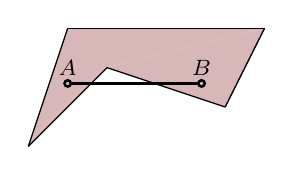
\begin{tikzpicture}
                        % \clip (0,0) rectangle (14.000000,10.000000);
                        {\footnotesize

                        % Changing color 215 183 183
                        \definecolor{r215g183b183}{rgb}{0.843137,0.717647,0.717647}%
                        \color{r215g183b183}% 

                        % Filling triangle C D G
                        \fill (1.500000,1.500000) -- (2.500000,2.500000) -- (2.000000,3.000000);%

                        % Filling triangle D E F
                        \fill (2.500000,2.500000) -- (4.000000,2.000000) -- (4.500000,3.000000);%

                        % Filling triangle D F G
                        \fill (2.500000,2.500000) -- (4.500000,3.000000) -- (2.000000,3.000000);%

                        % Changing color 0 0 0
                        \definecolor{r0g0b0}{rgb}{0.000000,0.000000,0.000000}%
                        \color{r0g0b0}% 

                        % Drawing segment C D
                        \draw [line width=0.016cm] (1.500000,1.500000) -- (2.500000,2.500000);%

                        % Drawing segment D E
                        \draw [line width=0.016cm] (2.500000,2.500000) -- (4.000000,2.000000);%

                        % Drawing segment E F
                        \draw [line width=0.016cm] (4.000000,2.000000) -- (4.500000,3.000000);%

                        % Drawing segment F G
                        \draw [line width=0.016cm] (4.500000,3.000000) -- (2.000000,3.000000);%

                        % Drawing segment G C
                        \draw [line width=0.016cm] (2.000000,3.000000) -- (1.500000,1.500000);%

                        % Marking point A by circle
                        \draw [line width=0.032cm] (2.000000,2.300000) circle (0.040000);%
                        \draw (2.000000,2.300000) node [anchor=south] { $A$ };%

                        % Marking point B by circle
                        \draw [line width=0.032cm] (3.700000,2.300000) circle (0.040000);%
                        \draw (3.700000,2.300000) node [anchor=south] { $B$ };%

                        % Drawing segment A B
                        \draw [line width=0.032cm] (2.040000,2.300000) -- (3.660000,2.300000);%
                        \color{black}
                        }
                    \end{tikzpicture}
                \end{figure}
            \end{multicols}   

        \end{definicija}
        

        ~
        
            \begin{definicija}
                Dva poltraka s skupnim izhodiščem določata dva \textbf{kota}.
                Izhodišče poltrakov imenujemo \textbf{vrh} kota, poltraka pa imenujemo \textbf{kraka} kota.
                
                \begin{figure}[H]
                    \centering
                    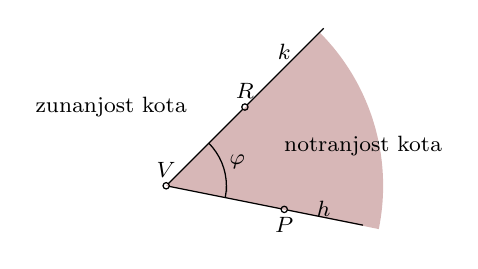
\begin{tikzpicture}
                        % \clip (0,0) rectangle (14.000000,10.000000);
                        {\footnotesize

                        % Changing color 215 183 183
                        \definecolor{r215g183b183}{rgb}{0.843137,0.717647,0.717647}%
                        \color{r215g183b183}% 

                        % Filling circle arc V B 56.31
                        \fill (2.500000,2.500000) -- (5.200000,1.949999) -- (5.204824,1.974235) arc (349:360:2.755449 and 2.755449) --(5.255449,2.500000) arc (0:44:2.755449 and 2.755449) -- (4.455318,4.441451) -- cycle;%

                        % Changing color 0 0 0
                        \definecolor{r0g0b0}{rgb}{0.000000,0.000000,0.000000}%
                        \color{r0g0b0}% 

                        % Drawing line V P
                        % \draw [line width=0.016cm] (1.000000,2.800000) -- (2.460777,2.507845);%
                        \draw [line width=0.016cm] (2.539223,2.492155) -- (3.960777,2.207845);%
                        \draw [line width=0.016cm] (4.039223,2.192155) -- (5.000000,2.000000);%

                        % Drawing line V R
                        % \draw [line width=0.016cm] (1.000000,1.000000) -- (2.471716,2.471716);%
                        \draw [line width=0.016cm] (2.528284,2.528284) -- (3.471716,3.471716);%
                        \draw [line width=0.016cm] (3.528284,3.528284) -- (4.500000,4.500000);%

                        % Marking point V by circle
                        \draw [line width=0.016cm] (2.500000,2.500000) circle (0.040000);%
                        \draw (2.500000,2.500000) node [anchor=south] { $V$ };%

                        % Marking point P by circle
                        \draw [line width=0.016cm] (4.000000,2.200000) circle (0.040000);%
                        \draw (4.000000,2.200000) node [anchor=north] { $P$ };%

                        % Marking point R by circle
                        \draw [line width=0.016cm] (3.500000,3.500000) circle (0.040000);%
                        \draw (3.500000,3.500000) node [anchor=south] { $R$ };%

                        % Marking point h
                        \draw (4.500000,2.000000) node [anchor=south] { $h$ };%

                        % Marking point k
                        \draw (4.000000,4.000000) node [anchor=south] { $k$ };%

                        % Drawing arc V A 56.31
                        \draw [line width=0.016cm] (3.250000,2.350000) -- (3.250800,2.354059) arc (349:360:0.764853 and 0.764853) --(3.264853,2.500000) arc (0:45:0.764853 and 0.764853);%

                        % Marking point \varphi
                        \draw (3.200000,2.800000) node [anchor=west] { $\varphi$ };%

                        % Marking point zun
                        \draw (1.800000,3.500000) node  { zunanjost kota };%

                        % Marking point not
                        \draw (5.000000,3.000000) node  { notranjost kota };%
                        \color{black}
                        }
                    \end{tikzpicture}
                \end{figure}
            \end{definicija}

            
                Če poltraka ne ležita na isti premici, je eden od kotov konveksen, drugi pa je nekonveksen.
            

            
                Kot lahko označimo na več načinov:
                \begin{itemize}
                    \item $\angle(h,k)$, kjer sta $h$ in $k$ poltraka, ki kot določata;
                    \item $\angle PVR$, kjer je $P$ točka na enem poltraku, $V$ vrh kota in $R$ točka na drugem poltraku;
                    \item $\alpha, \beta, \gamma, \dots$ -- z grškimi črkami.
                \end{itemize}
            
        
                ~

        
            \begin{definicija}
                Če poltraka s skupnim izhodiščem ležita na isti premici, vendar na različnih straneh izhodišča,
                določata dva enaka konveksna kota -- \textbf{iztegnjena kota}.

                \begin{figure}[H]
                    \centering
                    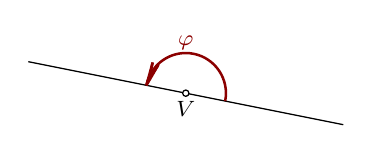
\begin{tikzpicture}
                        % \clip (0,0) rectangle (14.000000,10.000000);
                        {\footnotesize

                        % Drawing line V h
                        \draw [line width=0.016cm] (1.000000,2.000000) -- (2.960777,1.607845);%
                        \draw [line width=0.016cm] (3.039223,1.592155) -- (5.000000,1.200000);%

                        % Marking point V by circle
                        \draw [line width=0.016cm] (3.000000,1.600000) circle (0.040000);%
                        \draw (3.000000,1.600000) node [anchor=north] { $V$ };%

                        % Changing color 139 0 0
                        \definecolor{r139g0b0}{rgb}{0.545098,0.000000,0.000000}%
                        \color{r139g0b0}% 

                        % Drawing arc V h 180.00
                        \draw [line width=0.032cm] (3.500000,1.500000) -- (3.500534,1.502706) arc (349:360:0.509902 and 0.509902) --(3.509902,1.600000) arc (0:168:0.509902 and 0.509902) -- (2.500000,1.700000);%

                        % Marking point \varphi
                        \draw (3.000000,2.050000) node [anchor=south] { $\varphi$ };%

                        % Drawing arrow C A 1.00
                        \draw [line width=0.032cm] (2.651137,1.959148) -- (2.500000,1.700000);%
                        \draw [line width=0.032cm] (2.651137,1.959148) -- (2.538342,1.791430);%
                        \draw [line width=0.032cm] (2.578914,1.989435) -- (2.500000,1.700000);%
                        \draw [line width=0.032cm] (2.578914,1.989435) -- (2.538342,1.791430);%
                        \color{black}
                        }
                    \end{tikzpicture}
                \end{figure}
            \end{definicija}

            \begin{definicija}
                Če se poltraka na isti premici prekrivata, določata \textbf{polni kot} ali \textbf{ničelni kot}.

                \begin{figure}[H]
                    \centering
                    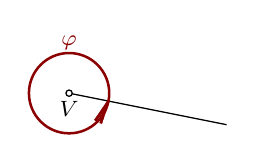
\begin{tikzpicture}
                        % \clip (0,0) rectangle (14.000000,10.000000);
                        {\footnotesize

                        % Drawing line V h
                        % \draw [line width=0.016cm] (1.000000,2.000000) -- (2.960777,1.607845);%
                        \draw [line width=0.016cm] (3.039223,1.592155) -- (5.000000,1.200000);%

                        % Marking point V by circle
                        \draw [line width=0.016cm] (3.000000,1.600000) circle (0.040000);%
                        \draw (3.000000,1.600000) node [anchor=north] { $V$ };%

                        % Changing color 139 0 0
                        \definecolor{r139g0b0}{rgb}{0.545098,0.000000,0.000000}%
                        \color{r139g0b0}% 

                        % Drawing arc V h 360.00
                        \draw [line width=0.032cm] (3.000000,1.600000) circle (0.509902);%

                        % Marking point \varphi
                        \draw (3.000000,2.050000) node [anchor=south] { $\varphi$ };%

                        % Drawing arrow k h 1.00
                        \draw [line width=0.032cm] (3.331960,1.251479) -- (3.500000,1.500000);%
                        \draw [line width=0.032cm] (3.331960,1.251479) -- (3.455661,1.411322);%
                        \draw [line width=0.032cm] (3.402008,1.216456) -- (3.500000,1.500000);%
                        \draw [line width=0.032cm] (3.402008,1.216456) -- (3.455661,1.411322);%
                        \color{black}
                        }
                    \end{tikzpicture} ~~~~~
                    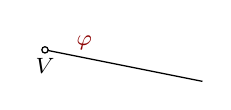
\begin{tikzpicture}
                        % \clip (0,0) rectangle (14.000000,10.000000);
                        {\footnotesize

                        % Drawing line V h
                        % \draw [line width=0.016cm] (1.000000,2.000000) -- (2.960777,1.607845);%
                        \draw [line width=0.016cm] (3.039223,1.592155) -- (5.000000,1.200000);%

                        % Marking point V by circle
                        \draw [line width=0.016cm] (3.000000,1.600000) circle (0.040000);%
                        \draw (3.000000,1.600000) node [anchor=north] { $V$ };%

                        % Changing color 139 0 0
                        \definecolor{r139g0b0}{rgb}{0.545098,0.000000,0.000000}%
                        \color{r139g0b0}% 

                        % Marking point \varphi
                        \draw (3.500000,1.500000) node [anchor=south] { $\varphi$ };%
                        \color{black}
                        }
                    \end{tikzpicture}
                \end{figure}

            \end{definicija}
        
            ~

        
            \begin{definicija}
                Kota s skupnim vrhom, ki imata en skupen krak, presek njunih notranjosti pa je prazen, sta \textbf{sosedna kota}.

                \begin{figure}[H]
                    \centering
                    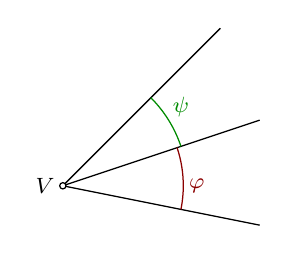
\begin{tikzpicture}
                        % \clip (0,0) rectangle (14.000000,10.000000);
                        {\footnotesize

                        % Drawing line V P
                        \draw [line width=0.016cm] (4.000000,1.000000) -- (1.539223,1.492155);%
                        % \draw [line width=0.016cm] (1.460777,1.507845) -- (1.000000,1.600000);%

                        % Drawing line V Q
                        % \draw [line width=0.016cm] (1.000000,1.333333) -- (1.462053,1.487351);%
                        \draw [line width=0.016cm] (1.537947,1.512649) -- (4.000000,2.333333);%

                        % Drawing line V R
                        % \draw [line width=0.016cm] (1.000000,1.000000) -- (1.471716,1.471716);%
                        \draw [line width=0.016cm] (1.528284,1.528284) -- (3.500000,3.500000);%

                        % Marking point V by circle
                        \draw [line width=0.016cm] (1.500000,1.500000) circle (0.040000);%
                        \draw (1.500000,1.500000) node [anchor=east] { $V$ };%

                        % Changing color 139 0 0
                        \definecolor{r139g0b0}{rgb}{0.545098,0.000000,0.000000}%
                        \color{r139g0b0}% 

                        % Drawing arc V P 29.74
                        \draw [line width=0.016cm] (3.000000,1.200000) -- (3.001601,1.208118) arc (349:360:1.529706 and 1.529706) --(3.029706,1.500000) arc (0:18:1.529706 and 1.529706) -- (2.951206,1.983735);%

                        % Marking point \varphi
                        \draw (3.200000,1.500000) node  { $\varphi$ };%

                        % Changing color 0 139 0
                        \definecolor{r0g139b0}{rgb}{0.000000,0.545098,0.000000}%
                        \color{r0g139b0}% 

                        % Drawing arc V Q 26.57
                        \draw [line width=0.016cm] (3.000000,2.000000) -- (2.994996,2.014768) arc (19:45:1.581139 and 1.581139);%

                        % Marking point \psi
                        \draw (3.000000,2.500000) node  { $\psi$ };%
                        \color{black}
                        }
                    \end{tikzpicture}
                \end{figure}
            \end{definicija}

            \begin{definicija}
                Sosedna kota, katerih kraka, ki  nista skupna, ležita na isti premici, sta \textbf{sokota}.
                
                \begin{figure}[H]
                    \centering
                    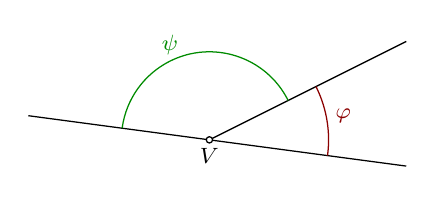
\begin{tikzpicture}
                        % \clip (0,0) rectangle (14.000000,10.000000);
                        {\footnotesize

                        % Drawing line V P
                        \draw [line width=0.016cm] (1.200000,1.806667) -- (3.460351,1.505287);%
                        \draw [line width=0.016cm] (3.539649,1.494713) -- (6.000000,1.166667);%

                        % Drawing line V Q
                        % \draw [line width=0.016cm] (2.700000,1.100000) -- (3.464223,1.482111);%
                        \draw [line width=0.016cm] (3.535777,1.517889) -- (6.000000,2.750000);%

                        % Marking point V by circle
                        \draw [line width=0.016cm] (3.500000,1.500000) circle (0.040000);%
                        \draw (3.500000,1.500000) node [anchor=north] { $V$ };%

                        % Changing color 139 0 0
                        \definecolor{r139g0b0}{rgb}{0.545098,0.000000,0.000000}%
                        \color{r139g0b0}% 

                        % Drawing arc V P 34.16
                        \draw [line width=0.016cm] (5.000000,1.300000) -- (5.001995,1.315578) arc (353:360:1.513275 and 1.513275) --(5.013275,1.500000) arc (0:26:1.513275 and 1.513275) -- (4.853514,2.176757);%

                        % Marking point \varphi
                        \draw (5.200000,1.800000) node  { $\varphi$ };%

                        % Changing color 0 139 0
                        \definecolor{r0g139b0}{rgb}{0.000000,0.545098,0.000000}%
                        \color{r0g139b0}% 

                        % Drawing arc V Q 145.84
                        \draw [line width=0.016cm] (4.500000,2.000000) -- (4.496176,2.007577) arc (27:172:1.118034 and 1.118034) -- (2.391774,1.647764);%

                        % Marking point \psi
                        \draw (3.000000,2.700000) node  { $\psi$ };%
                        \color{black}
                        }
                    \end{tikzpicture}
                \end{figure}
            \end{definicija}

        

            ~\\
        
            \begin{definicija}
                Tri nekolinearne točke $A$, $B$ in $C$ določajo \textbf{trikotnik} $\triangle ABC$.
                Točke $A$, $B$ in $C$ so \textbf{oglišča} trikotnika, daljice $AB$, $BC$ in $AC$ so njegove \textbf{stranice}.

            \begin{figure}[H]
                \centering
                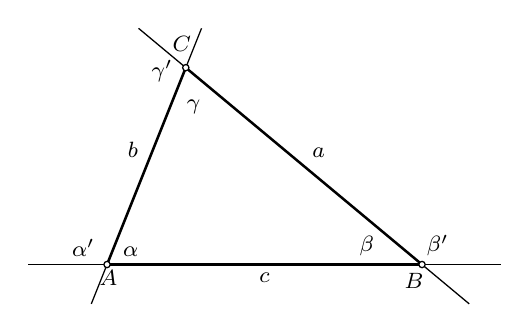
\begin{tikzpicture}
                    % \clip (0,0) rectangle (14.000000,10.000000);
                    {\footnotesize
                    
                    % Marking point A by circle
                    \draw [line width=0.016cm] (2.000000,1.500000) circle (0.040000);%
                    \draw (1.800000,1.530000) node [anchor=north west] { $A$ };%
                    
                    % Marking point B by circle
                    \draw [line width=0.016cm] (6.000000,1.500000) circle (0.040000);%
                    \draw (5.900000,1.500000) node [anchor=north] { $B$ };%
                    
                    % Marking point C by circle
                    \draw [line width=0.016cm] (3.000000,4.000000) circle (0.040000);%
                    \draw (2.950000,4.100000) node [anchor=south] { $C$ };%
                    
                    % Drawing line A B
                    \draw [line width=0.016cm] (1.000000,1.500000) -- (1.960000,1.500000);%
                    \draw [line width=0.016cm] (2.040000,1.500000) -- (5.960000,1.500000);%
                    \draw [line width=0.016cm] (6.040000,1.500000) -- (7.000000,1.500000);%
                    
                    % Drawing line B C
                    \draw [line width=0.016cm] (6.600000,1.000000) -- (6.030729,1.474393);%
                    \draw [line width=0.016cm] (5.969271,1.525607) -- (3.030729,3.974393);%
                    \draw [line width=0.016cm] (2.969271,4.025607) -- (2.400000,4.500000);%
                    
                    % Drawing line A C
                    \draw [line width=0.016cm] (1.800000,1.000000) -- (1.985144,1.462861);%
                    \draw [line width=0.016cm] (2.014856,1.537139) -- (2.985144,3.962861);%
                    \draw [line width=0.016cm] (3.014856,4.037139) -- (3.200000,4.500000);%
                    
                    % Marking point c
                    \draw (4.000000,1.500000) node [anchor=north] { $c$ };%
                    
                    % Marking point a
                    \draw (4.500000,2.750000) node [anchor=south west] { $a$ };%
                    
                    % Marking point b
                    \draw (2.500000,2.750000) node [anchor=south east] { $b$ };%
                    
                    % Marking point \gamma
                    \draw (3.100000,3.700000) node [anchor=north] { $\gamma$ };%
                    
                    % Marking point \gamma'
                    \draw (2.700000,4.200000) node [anchor=north] { $\gamma'$ };%
                    
                    % Marking point \beta
                    \draw (5.300000,1.500000) node [anchor=south] { $\beta$ };%
                    
                    % Marking point \beta'
                    \draw (6.200000,1.500000) node [anchor=south] { $\beta'$ };%
                    
                    % Marking point \alpha
                    \draw (2.300000,1.500000) node [anchor=south] { $\alpha$ };%
                    
                    % Marking point \alpha'
                    \draw (1.700000,1.500000) node [anchor=south] { $\alpha'$ };%
                    
                    % Drawing segment A B
                    \draw [line width=0.032cm] (2.040000,1.500000) -- (5.960000,1.500000);%
                    
                    % Drawing segment B C
                    \draw [line width=0.032cm] (5.969271,1.525607) -- (3.030729,3.974393);%
                    
                    % Drawing segment A C
                    \draw [line width=0.032cm] (2.014856,1.537139) -- (2.985144,3.962861);%
                    }
                \end{tikzpicture}
            \end{figure}

                Koti $\alpha$, $\beta$ in $\gamma$ so \textbf{notranji koti}, 
                njihovi sokoti $\alpha'$, $\beta'$ in $\gamma'$ pa so \textbf{zunanji koti} trikotnika.

            \end{definicija}

            
                Trikotnik je \textbf{pozitivno orientiran}, če si njegova oglišča sledijo v nasprotni smeri vrtenja urnega kazalca; 
                če si sledijo v smeri vrtenja urnega kazalca, pa je \textbf{negativno orientiran}.
            
        
            ~

        
            \begin{definicija}
                Točke $A_1, A_2, A_3, \dots, A_n$ v ravnini, od katerih nobene zaporedne tri niso kolinearne, določajo \textbf{$n$-kotnik}.
                Točke $A_1, A_2, A_3, \dots, A_n$ so \textbf{oglišča} $n$-kotnika;
                daljice, ki povezujejo sosedni oglišči, $A_1A_2, A_2A_3, \dots, A_nA_1$ so \textbf{stranice} $n$-kotnika;
                daljice, ki povezujejo po dve nesosedni oglišči, pa so \textbf{diagonale} $n$-kotnika.
            \end{definicija}

            
                Poljuben $n$-kotnika ima $$\dfrac{n(n-3)}{2}$$ diagonal -- iz vsakega od $n$ oglišč gre $n-3$ diagonal, vsaka pa je šteta dvakrat.
            
            ~
            
                Če za vsako nosilko stranice $n$-kotnika velja, da preostala oglišča ležijo na isti strani te nosilke, je $n$-kotnik \textbf{konveksen}.
            
        




        %%%%% naloge

        ~\\~\\

            \begin{naloga}
                Izračunajte število diagonal: $17$-kotnika, $31$-kotnika in $28$-kotnika.                
            \end{naloga}

            \begin{naloga}
                Ugotovite, ali obstaja $n$-kotnik, ki ima desetino toliko diagonal kot $28$-kotnik.
                Če obstaja, izračunajte, koliko stranic ima.
            \end{naloga}   
            
            \begin{naloga}
                Kateri $n$-kotnik ima štirikrat toliko diagonal kot stranic?
            \end{naloga}
        
            \begin{naloga}
                Izračunajte, kateri $n$-kotnik ima: $104$ diagonale, $230$ diagonal, $2n-5$ diagonal.
            \end{naloga}

            \begin{naloga}
                Pokažite, da ne obstaja $n$-kotnik, ki ima $13$ diagonal.  
            \end{naloga}
            

            \begin{naloga}
                Za vsako od spodnjih izjav ugotovite, ali je pravilna ali nepravilna.
                \begin{itemize}
                    \item Tri različne točke, so vedno nekolinearne.
                    \item Petkotnik ima enako število diagonal in stranic.
                    \item Štiri različne premice se sekajo v največ $4$ različnih točkah.
                    \item Skozi štiri kolinearne točke gredo tri različne premice.
                    \item Vzporedni premici imata lahko neskončno mnogo skupnih točk.
                \end{itemize}
            \end{naloga}

            \begin{naloga}
                Pokažite, da je število diagonal $25$-kotnika večkratnik števila njegovih stranic.
            \end{naloga}

            \begin{naloga}
                Vsota števila stranic in diagonal $n$-kotnika je $105$? Kateri $n$-kotnik je to?
            \end{naloga}
        

            \begin{naloga}
                Izračunajte, kateri $n$-kotnik ima toliko diagonal kot stranic.
            \end{naloga}

            \begin{naloga}
                Člani filatelističnega društva so se domenili, da si bodo za praznike spet pošiljali voščilnice po klasični pošti.
                Ko so se dobili po novem letu, so prinesli vse voščilnice in jih našteli $132$.
                Izračunajte, koliko članov društva, si je medseboj poslalo voščilnice.                
            \end{naloga}


        

\newpage
%%%%%%%%%%%%%%%%%%%%%%%%%%%%%%%%%%%%%%%


\section{Skladnost in merjenje}


    \begin{definicija}
        Dva lika $L$ in $L'$ sta \textbf{skladna}, če lahko lik $L$ prenesemo na lik $L'$ tako,
        da se popolnoma prekrijeta.

        Znak za skladnost je $\cong$.
    \end{definicija}

    
        \textbf{Skladnost} je v množici ravninskih likov \textit{ekvivalenčna relacija}, saj je:
        \begin{itemize}
            \item \textit{refleksivna}: $L\cong L$ -- vsaka množica je skladna sama s seboj;
            \item \textit{simetrična}: $L\cong L' \Rightarrow L'\cong L$ -- če je prva množica skladna z drugo, je tudi druga skladna s prvo;
            \item \textit{tranzitivna}: $L\cong L' \land L'\cong L'' \rightarrow L\cong L''$ -- če je prva množica skladna z drugo in druga skladna s tretjo, 
                    je tudi prva množica skladna s tretjo množico.
        \end{itemize}
    

~


    \begin{definicija}
        Kot, ki je skladen s svojim sokotom, je \textbf{pravi kot}.

        \begin{figure}[H]
            \centering
            \begin{tikzpicture}
            % \clip (0,0) rectangle (14.000000,10.000000);
            {\footnotesize

            % Drawing line V A
            \draw [line width=0.016cm] (1.000000,1.500000) -- (2.960000,1.500000);%
            \draw [line width=0.016cm] (3.040000,1.500000) -- (5.000000,1.500000);%

            % Drawing line V B
            % \draw [line width=0.016cm] (3.000000,1.000000) -- (3.000000,1.460000);%
            \draw [line width=0.016cm] (3.000000,1.540000) -- (3.000000,3.500000);%

            % Marking point V by circle
            \draw [line width=0.016cm] (3.000000,1.500000) circle (0.040000);%

            % Changing color 139 0 0
            \definecolor{r139g0b0}{rgb}{0.545098,0.000000,0.000000}%
            \color{r139g0b0}% 

            % Drawing arc V A 90.00
            \draw [line width=0.032cm] (3.800000,1.500000) arc (360:360:0.800000 and 0.800000) --(3.800000,1.500000) arc (0:90:0.800000 and 0.800000);%

            % Changing color 0 139 0
            \definecolor{r0g139b0}{rgb}{0.000000,0.545098,0.000000}%
            \color{r0g139b0}% 

            % Drawing arc V B 90.00
            \draw [line width=0.032cm] (3.000000,2.200000) arc (90:180:0.700000 and 0.700000);%
            \color{black}
            }
            \end{tikzpicture}

        \end{figure}
        
    \end{definicija}

    
        Če si kraka sledita v nasprotni smeri vrtenja urnega kazalca, je \textbf{orientacija kota pozitivna}, 
        če pa si sledita v smeri vrtenja urnega kazalca, pa je \textbf{orientacija kota negativna}.

        \begin{figure}[H]
                \centering
            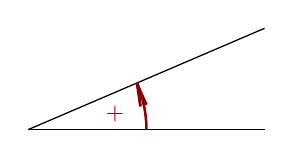
\begin{tikzpicture}
            % \clip (0,0) rectangle (14.000000,10.000000);
            {\footnotesize

            % Drawing segment A b
            \draw [line width=0.016cm] (1.500000,1.500000) -- (4.500000,1.500000);%

            % Drawing segment A C
            \draw [line width=0.016cm] (1.500000,1.500000) -- (4.500000,2.785714);%

            % Changing color 139 0 0
            \definecolor{r139g0b0}{rgb}{0.545098,0.000000,0.000000}%
            \color{r139g0b0}% 

            % Drawing arc A B 23.20
            \draw [line width=0.032cm] (3.000000,1.500000) arc (360:360:1.500000 and 1.500000) --(3.000000,1.500000) arc (0:23:1.500000 and 1.500000) -- (2.878718,2.090879);%

            % Drawing arrow Bb U 1.00
            \draw [line width=0.032cm] (2.923918,1.794304) -- (2.878718,2.090879);%
            \draw [line width=0.032cm] (2.923918,1.794304) -- (2.906321,1.995655);%
            \draw [line width=0.032cm] (2.999137,1.816108) -- (2.878718,2.090879);%
            \draw [line width=0.032cm] (2.999137,1.816108) -- (2.906321,1.995655);%

            % Marking point +
            \draw (2.600000,1.700000) node  { $+$ };%
            \color{black}
            }
            \end{tikzpicture} ~~~~~
            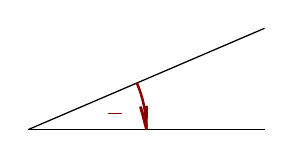
\begin{tikzpicture}
            % \clip (0,0) rectangle (14.000000,10.000000);
            {\footnotesize

            % Drawing segment A b
            \draw [line width=0.016cm] (1.500000,1.500000) -- (4.500000,1.500000);%

            % Drawing segment A C
            \draw [line width=0.016cm] (1.500000,1.500000) -- (4.500000,2.785714);%

            % Changing color 139 0 0
            \definecolor{r139g0b0}{rgb}{0.545098,0.000000,0.000000}%
            \color{r139g0b0}% 

            % Drawing arc A B 23.20
            \draw [line width=0.032cm] (3.000000,1.500000) arc (360:360:1.500000 and 1.500000) --(3.000000,1.500000) arc (0:23:1.500000 and 1.500000) -- (2.878718,2.090879);%

            % Drawing arrow Bb B 1.00
            \draw [line width=0.032cm] (3.001963,1.799994) -- (3.000000,1.500000);%
            \draw [line width=0.032cm] (3.001963,1.799994) -- (2.987703,1.598379);%
            \draw [line width=0.032cm] (2.924252,1.790280) -- (3.000000,1.500000);%
            \draw [line width=0.032cm] (2.924252,1.790280) -- (2.987703,1.598379);%

            % Marking point -
            \draw (2.600000,1.700000) node  { $-$ };%
            \color{black}
            }
            \end{tikzpicture}
        \end{figure}
    




        ~

    
        Daljici $AB$ in $CD$, ki nista skladni, lahko premaknemo na poljubni premici tako,
        da levi krajišči sovpadata in da eno od desnih krajišč, npr. $D$ leži med $A$ in $B$.
        V tem primeru je daljica $AB$ \textbf{daljša} od daljice $CD$ oziroma je daljica $CD$ \textbf{krajša} od daljice $AB$.
    

    \begin{aksiom}[Arhimedov aksiom]
        Obstaja tako naravno število $n$, pri katerem je vsota $n$ krajših daljic $CD$ daljša od daljice $AB$,
        vsota $n-1$ krajših daljic $CD$ pa je kvečjemu skladna z daljico $AB$.
        $$n\cdot |CD|>|AB| \quad \quad (n-1)\cdot |CD|\leq |AB|$$

        \begin{figure}[H]
            \centering
            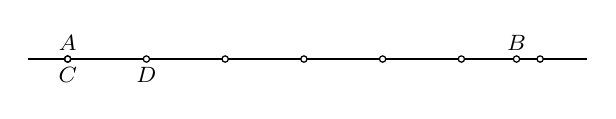
\begin{tikzpicture}
            % \clip (0,0) rectangle (14.000000,10.000000);
            {\footnotesize

            % Drawing line A B
            \draw [line width=0.016cm] (1.000000,1.500000) -- (1.460000,1.500000);%
            \draw [line width=0.016cm] (1.540000,1.500000) -- (2.460000,1.500000);%
            \draw [line width=0.016cm] (2.540000,1.500000) -- (3.460000,1.500000);%
            \draw [line width=0.016cm] (3.540000,1.500000) -- (4.460000,1.500000);%
            \draw [line width=0.016cm] (4.540000,1.500000) -- (5.460000,1.500000);%
            \draw [line width=0.016cm] (5.540000,1.500000) -- (6.460000,1.500000);%
            \draw [line width=0.016cm] (6.540000,1.500000) -- (7.160000,1.500000);%
            \draw [line width=0.016cm] (7.240000,1.500000) -- (7.460000,1.500000);%
            \draw [line width=0.016cm] (7.540000,1.500000) -- (8.100000,1.500000);%

            % Marking point A by circle
            \draw [line width=0.016cm] (1.500000,1.500000) circle (0.040000);%
            \draw (1.500000,1.500000) node [anchor=south] { $A$ };%

            % Marking point B by circle
            \draw [line width=0.016cm] (7.200000,1.500000) circle (0.040000);%
            \draw (7.200000,1.500000) node [anchor=south] { $B$ };%

            % Marking point C by circle
            \draw [line width=0.016cm] (1.500000,1.500000) circle (0.040000);%
            \draw (1.500000,1.500000) node [anchor=north] { $C$ };%

            % Marking point D by circle
            \draw [line width=0.016cm] (2.500000,1.500000) circle (0.040000);%
            \draw (2.500000,1.500000) node [anchor=north] { $D$ };%

            % Marking point E by circle
            \draw [line width=0.016cm] (3.500000,1.500000) circle (0.040000);%

            % Marking point F by circle
            \draw [line width=0.016cm] (4.500000,1.500000) circle (0.040000);%

            % Marking point G by circle
            \draw [line width=0.016cm] (5.500000,1.500000) circle (0.040000);%

            % Marking point H by circle
            \draw [line width=0.016cm] (6.500000,1.500000) circle (0.040000);%

            % Marking point I by circle
            \draw [line width=0.016cm] (7.500000,1.500000) circle (0.040000);%
            }
            \end{tikzpicture}
        \end{figure}
    \end{aksiom}

    % 
        Daljico $CD$, s katero smo izmerili daljico $AB$, imenujemo \textbf{enotska daljica}.
        Tako smo daljici $AB$ priredili natančno določeno število -- \textbf{dolžino} daljice $AB$ oziroma \textbf{razdaljo} točk $A$ in $B$.
        $$ |AB|=d(A,B)$$
    % 
    
        % Daljico $CD$ imenujemo \textbf{enotska daljica}.
        % Daljici $AB$ smo priredili natančno določeno število -- \textbf{dolžino} daljice $AB$ oziroma \textbf{razdaljo} točk $A$ in $B$.

        % $$ |AB|=d(A,B)$$
    





    \begin{aksiom}
        Če je $AB$ poljubna daljica, $A'$ pa točka na poljubnem poltraku, obstaja na tem poltraku natančno določena točka $B'$,
        da je daljica $A'B'$ skladna z daljico $AB$.

        $$A'B'\cong AB$$
    \end{aksiom}

    \begin{izrek}
        Skladni daljici imata enako dolžino.
        % $$|A'B'|=|AB|$$
    \end{izrek}

    ~ 

    \begin{aksiom}
        Naj daljici $AB$ in $BC$ ležita na isti premici in naj imata skupno le točko $B$.
        Daljici $A'B'$ in $B'C'$ naj ležita na tej ali neki drugi premici in naj imata skupno točko $B'$.
        Če velja $AB\cong A'B'$ in $BC\cong B'C'$, potem velja tudi $AC\cong A'C'$.
    \end{aksiom}

    \begin{izrek}
        Dolžina vsote daljic je enaka vsoti dolžin posameznih daljic.
    \end{izrek}




    \subsection*{Enote}


    
        Osnovna enota za merjenje dolžine je \textbf{meter}.

        Iz nje izpeljane enote pa so \textit{decimeter}, \textit{centimeter}, \textit{milimeter}, \textit{kilometer} itd.
        $$ 1~m=10~dm=100~cm=1000~mm$$  $$1~km=1000~m$$ 
    

    
        Enota za merjenje kotov je \textbf{kotna stopinja} -- velikost $\dfrac{1}{360}$ polnega kota.
        
        Izpeljani enoti sta \textit{(kotna) minuta} in \textit{(kotna) sekunda}.
        $$1^\circ=60'=3600''$$ 
    

    
        Velikost kota nič je $0^\circ$, pravega kota je $90^\circ$, iztegnjenega kota je $180^\circ$, polnega kota pa je $360^\circ$.
    

~


    \begin{definicija}
        Kota $\varphi$ in $\psi$, katerih vsota meri $180^\circ$, sta \textbf{suplementarna kota}.

        \begin{figure}[H]
            \centering
            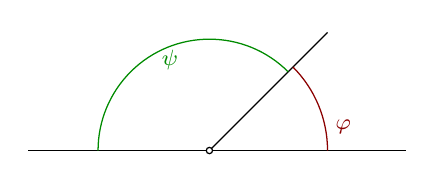
\begin{tikzpicture}
            % \clip (0,0) rectangle (14.000000,10.000000);
            {\footnotesize

            % Drawing line V P
            \draw [line width=0.016cm] (1.200000,1.500000) -- (3.460000,1.500000);%
            \draw [line width=0.016cm] (3.540000,1.500000) -- (6.000000,1.500000);%

            % Drawing line V Q
            % \draw [line width=0.016cm] (3.100000,1.100000) -- (3.471716,1.471716);%
            \draw [line width=0.016cm] (3.528284,1.528284) -- (5.000000,3.000000);%

            % Marking point V by circle
            \draw [line width=0.016cm] (3.500000,1.500000) circle (0.040000);%

            % Changing color 139 0 0
            \definecolor{r139g0b0}{rgb}{0.545098,0.000000,0.000000}%
            \color{r139g0b0}% 

            % Drawing arc V P 45.00
            \draw [line width=0.016cm] (5.000000,1.500000) arc (360:360:1.500000 and 1.500000) --(5.000000,1.500000) arc (0:45:1.500000 and 1.500000);%

            % Marking point \varphi
            \draw (5.200000,1.80000) node  { $\varphi$ };%

            % Changing color 0 139 0
            \definecolor{r0g139b0}{rgb}{0.000000,0.545098,0.000000}%
            \color{r0g139b0}% 

            % Drawing arc V Q 135.00
            \draw [line width=0.016cm] (4.500000,2.500000) arc (45:180:1.414214 and 1.414214);%

            % Marking point \psi
            \draw (3.000000,2.650000) node  { $\psi$ };%
            \color{black}
            }
            \end{tikzpicture}
        \end{figure}
    \end{definicija}

                
    \begin{definicija}
        Kota $\varphi$ in $\psi$, katerih vsota meri $90^\circ$, sta \textbf{komplementarna kota}.

        \begin{figure}[H]
            \centering
            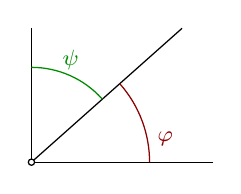
\begin{tikzpicture}
            % \clip (0,0) rectangle (14.000000,10.000000);
            {\footnotesize

            % Drawing line V P
            % \draw [line width=0.016cm] (2.800000,1.500000) -- (3.460000,1.500000);%
            \draw [line width=0.016cm] (3.540000,1.500000) -- (5.800000,1.500000);%

            % Drawing line V Q
            % \draw [line width=0.016cm] (3.050000,1.100000) -- (3.470104,1.473425);%
            \draw [line width=0.016cm] (3.529896,1.526575) -- (5.412500,3.200000);%

            % Drawing line V R
            % \draw [line width=0.016cm] (3.500000,1.100000) -- (3.500000,1.460000);%
            \draw [line width=0.016cm] (3.500000,1.540000) -- (3.500000,3.200000);%

            % Marking point V by circle
            \draw [line width=0.016cm] (3.500000,1.500000) circle (0.040000);%

            % Changing color 139 0 0
            \definecolor{r139g0b0}{rgb}{0.545098,0.000000,0.000000}%
            \color{r139g0b0}% 

            % Drawing arc V P 41.63
            \draw [line width=0.016cm] (5.000000,1.500000) arc (360:360:1.500000 and 1.500000) --(5.000000,1.500000) arc (0:41:1.500000 and 1.500000) -- (4.621114,2.496546);%

            % Marking point \varphi
            \draw (5.200000,1.800000) node  { $\varphi$ };%

            % Changing color 0 139 0
            \definecolor{r0g139b0}{rgb}{0.000000,0.545098,0.000000}%
            \color{r0g139b0}% 

            % Drawing arc V Q 48.37
            \draw [line width=0.016cm] (4.400000,2.300000) -- (4.394865,2.305740) arc (42:90:1.204159 and 1.204159);%

            % Marking point \psi
            \draw (4.000000,2.800000) node  { $\psi$ };%
            \color{black}
            }
            \end{tikzpicture}
        \end{figure}
    \end{definicija}

    
        Sokota sta vedno suplementarna kota.
    




    \subsection*{Skladnost trikotnikov}


    \begin{definicija}
        Dva trikotnika sta \textbf{skladna}, če imata paroma skladne vse stranice in tem stranicam nasprotne kote.
    \end{definicija}

    \begin{aksiom}
        Dva trikotnika sta skladna, če se ujemata v dveh stranicah in v vmesnem kotu.
    \end{aksiom}

    \begin{izrek}
        Trikotnika $\triangle ABC$ in $\triangle A'B'C'$ sta skladna, če se ujemata:
        \begin{enumerate}
            \item v vseh treh stranicah;
            \item v eni stranici in obeh priležnih kotih;
            \item v dveh stranicah in kotu, ki leži nasproti daljši od obeh stranic.
        \end{enumerate}
    \end{izrek}




%%%% naloge


~\\~~\\~\\


    \begin{naloga}
        Izračunajte dolžino daljice, če ena polovica meri $2x-7$ enot, druga polovica pa $x+8$ enot.
    \end{naloga}

    \begin{naloga}
        Izračunaj dolžino $x$ daljice $AB$, če je točka $S$ njeno razpolovišče, točka $R$ pa razpolovišče daljice $SB$ in je $\lvert SR \rvert = \dfrac{x}{3}-1$.
    \end{naloga}

    \begin{naloga}
        Izračunajte velikosti kotov $\angle AVM$ in $\angle FVE$, če poltrak $VM$ obakrat razpolavlja kot.

        \begin{figure}[H]
            \centering
            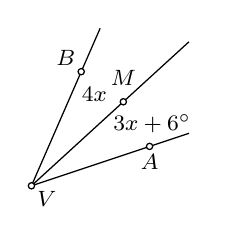
\begin{tikzpicture}
                % \clip (0,0) rectangle (14.000000,10.000000);
                {\footnotesize

                % Marking point V by circle
                \draw [line width=0.016cm] (1.500000,1.500000) circle (0.040000);%
                \draw (1.470000,1.530000) node [anchor=north west] { $V$ };%

                % Marking point A by circle
                \draw [line width=0.016cm] (3.000000,2.000000) circle (0.040000);%
                \draw (3.000000,2.000000) node [anchor=north] { $A$ };%

                % Drawing line V A
                % \draw [line width=0.016cm] (1.200000,1.400000) -- (1.462053,1.487351);%
                \draw [line width=0.016cm] (1.537947,1.512649) -- (2.962053,1.987351);%
                \draw [line width=0.016cm] (3.037947,2.012649) -- (3.500000,2.166667);%

                % Marking point M by circle
                \draw [line width=0.016cm] (2.666950,2.566878) circle (0.040000);%
                \draw (2.666950,2.666878) node [anchor=south] { $M$ };%

                % Marking point B by circle
                \draw [line width=0.016cm] (2.132124,2.949283) circle (0.040000);%
                \draw (2.162124,2.919283) node [anchor=south east] { $B$ };%

                % Drawing line V B
                % \draw [line width=0.016cm] (1.369151,1.200000) -- (1.484008,1.463336);%
                \draw [line width=0.016cm] (1.515992,1.536664) -- (2.116132,2.912618);%
                \draw [line width=0.016cm] (2.148115,2.985947) -- (2.372326,3.500000);%

                % Drawing line V M
                % \draw [line width=0.016cm] (1.200000,1.225727) -- (1.470478,1.473010);%
                \draw [line width=0.016cm] (1.529522,1.526990) -- (2.637428,2.539888);%
                \draw [line width=0.016cm] (2.696472,2.593868) -- (3.500000,3.328489);%

                % Marking point {3x+6^\circ}
                \draw (3.033475,2.283439) node  { ${3x+6^\circ}$ };%

                % Marking point {4x}
                \draw (2.299537,2.658080) node  { ${4x}$ };%
                }
            \end{tikzpicture} ~
            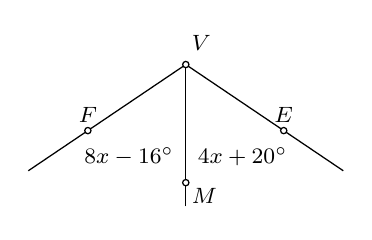
\begin{tikzpicture}
                % \clip (0,0) rectangle (14.000000,10.000000);
                {\footnotesize

                % Marking point V by circle
                \draw [line width=0.016cm] (4.000000,4.000000) circle (0.040000);%
                \draw (3.970000,4.070000) node [anchor=south west] { $V$ };%

                % Marking point M by circle
                \draw [line width=0.016cm] (4.000000,2.500000) circle (0.040000);%
                \draw (3.970000,2.530000) node [anchor=north west] { $M$ };%

                % Drawing line V M
                \draw [line width=0.016cm] (4.000000,2.200000) -- (4.000000,2.460000);%
                \draw [line width=0.016cm] (4.000000,2.540000) -- (4.000000,3.960000);%
                % \draw [line width=0.016cm] (4.000000,4.040000) -- (4.000000,4.200000);%

                % Marking point F by circle
                \draw [line width=0.016cm] (2.756444,3.161211) circle (0.040000);%
                \draw (2.756444,3.161211) node [anchor=south] { $F$ };%

                % Marking point E by circle
                \draw [line width=0.016cm] (5.243556,3.161211) circle (0.040000);%
                \draw (5.243556,3.161211) node [anchor=south] { $E$ };%

                % Drawing line V E
                % \draw [line width=0.016cm] (3.703488,4.200000) -- (3.966838,4.022368);%
                \draw [line width=0.016cm] (4.033162,3.977632) -- (5.210395,3.183578);%
                \draw [line width=0.016cm] (5.276718,3.138843) -- (6.000000,2.650983);%

                % Drawing line V F
                % \draw [line width=0.016cm] (4.296512,4.200000) -- (4.033162,4.022368);%
                \draw [line width=0.016cm] (3.966838,3.977632) -- (2.789605,3.183578);%
                \draw [line width=0.016cm] (2.723282,3.138843) -- (2.000000,2.650983);%

                % Marking point {8x-16^\circ}
                \draw (3.278222,2.830605) node  { ${8x-16^\circ}$ };%

                % Marking point {4x+20^\circ}
                \draw (4.721778,2.830605) node  { ${4x+20^\circ}$ };%
                }
            \end{tikzpicture}


        \end{figure}
    \end{naloga}


    \begin{multicols}{2}
    \begin{naloga}
        Izračunajte velikosti kotov $\alpha$ in $\beta$, če je $\alpha=\beta$.
        Podatke razberite s skice.

        \begin{figure}[H]
            \centering
            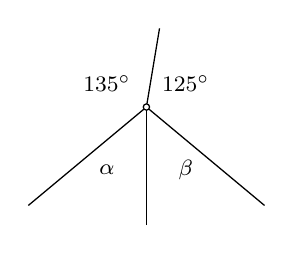
\begin{tikzpicture}
                % \clip (0,0) rectangle (14.000000,10.000000);
                {\footnotesize

                % Marking point A by circle
                \draw [line width=0.016cm] (3.000000,3.000000) circle (0.040000);%

                % Drawing segment A B
                \draw [line width=0.016cm] (3.000000,1.500000) -- (3.000000,2.960000);%

                % Drawing segment A C
                \draw [line width=0.016cm] (3.030729,2.974393) -- (4.500000,1.750000);%

                % Drawing segment A D
                \draw [line width=0.016cm] (2.969271,2.974393) -- (1.500000,1.750000);%

                % Drawing segment A E
                \draw [line width=0.016cm] (3.006576,3.039456) -- (3.166667,4.000000);%

                % Marking point \beta
                \draw (3.500000,2.200000) node  { $\beta$ };%

                % Marking point \alpha
                \draw (2.500000,2.200000) node  { $\alpha$ };%

                % Marking point {125^\circ}
                \draw (3.500000,3.300000) node  { ${125^\circ}$ };%

                % Marking point {135^\circ}
                \draw (2.500000,3.300000) node  { ${135^\circ}$ };%
                }
            \end{tikzpicture}

        \end{figure}
    \end{naloga}




    \begin{naloga}
        Iz podatkov na skici izračunajte neznano velikost kota $x$.

        \begin{figure}[H]
            \centering
            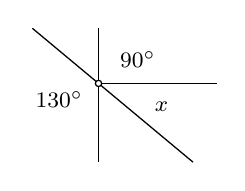
\begin{tikzpicture}
                % \clip (0,0) rectangle (14.000000,10.000000);
                {\footnotesize

                % Marking point A by circle
                \draw [line width=0.016cm] (3.000000,3.000000) circle (0.040000);%

                % Drawing line A B
                \draw [line width=0.016cm] (3.000000,2.000000) -- (3.000000,2.960000);%
                \draw [line width=0.016cm] (3.000000,3.040000) -- (3.000000,3.700000);%

                % Drawing line A C
                \draw [line width=0.016cm] (4.200000,2.000000) -- (3.030729,2.974393);%
                \draw [line width=0.016cm] (2.969271,3.025607) -- (2.160000,3.700000);%

                % Drawing segment A E
                \draw [line width=0.016cm] (3.040000,3.000000) -- (4.500000,3.000000);%

                % Marking point x
                \draw (3.800000,2.700000) node  { $x$ };%

                % Marking point {90^\circ}
                \draw (3.500000,3.300000) node  { ${90^\circ}$ };%

                % Marking point {130^\circ}
                \draw (2.500000,2.800000) node  { ${130^\circ}$ };%
                }
            \end{tikzpicture}

        \end{figure}
    \end{naloga}

\end{multicols}





    \begin{multicols}{2}
        
    \begin{naloga}
        Izračunajte velikost kota $\angle PVQ$, če je $\angle PVR=94^\circ$.

        \begin{figure}[H]
            \centering
            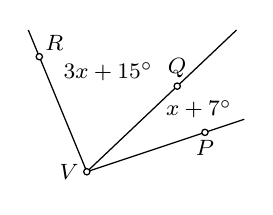
\begin{tikzpicture}
                % \clip (0,0) rectangle (14.000000,10.000000);
                {\footnotesize

                % Marking point V by circle
                \draw [line width=0.016cm] (3.500000,1.500000) circle (0.040000);%
                \draw (3.500000,1.500000) node [anchor=east] { $V$ };%

                % Marking point P by circle
                \draw [line width=0.016cm] (5.000000,2.000000) circle (0.040000);%
                \draw (5.000000,2.000000) node [anchor=north] { $P$ };%

                % Drawing line V P
                % \draw [line width=0.016cm] (2.600000,1.200000) -- (3.462053,1.487351);%
                \draw [line width=0.016cm] (3.537947,1.512649) -- (4.962053,1.987351);%
                \draw [line width=0.016cm] (5.037947,2.012649) -- (5.500000,2.166667);%

                % Marking point Q by circle
                \draw [line width=0.016cm] (4.648153,2.587081) circle (0.040000);%
                \draw (4.648153,2.587081) node [anchor=south] { $Q$ };%

                % Marking point R by circle
                \draw [line width=0.016cm] (2.896583,2.961468) circle (0.040000);%
                \draw (2.866583,2.931468) node [anchor=south west] { $R$ };%

                % Drawing line V R
                % \draw [line width=0.016cm] (3.623865,1.200000) -- (3.515265,1.463027);%
                \draw [line width=0.016cm] (3.484735,1.536973) -- (2.911849,2.924495);%
                \draw [line width=0.016cm] (2.881318,2.998440) -- (2.756809,3.300000);%

                % Drawing line V Q
                % \draw [line width=0.016cm] (3.183146,1.200000) -- (3.470954,1.472499);%
                \draw [line width=0.016cm] (3.529046,1.527501) -- (4.619106,2.559580);%
                \draw [line width=0.016cm] (4.677199,2.614582) -- (5.401122,3.300000);%

                % Marking point {x+7^\circ}
                \draw (4.924076,2.293541) node  { ${x+7^\circ}$ };%

                % Marking point {3x+15^\circ}
                \draw (3.772368,2.774275) node  { ${3x+15^\circ}$ };%
                }
            \end{tikzpicture}

        \end{figure}
    \end{naloga}


    \begin{naloga}
        Izračunajte velikost kota $\angle SVR$, če je $\angle QVS=50^\circ$.

        \begin{figure}[H]
            \centering
            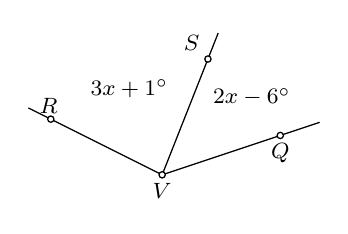
\begin{tikzpicture}
                % \clip (0,0) rectangle (14.000000,10.000000);
                {\footnotesize

                % Marking point V by circle
                \draw [line width=0.016cm] (3.500000,1.500000) circle (0.040000);%
                \draw (3.500000,1.500000) node [anchor=north] { $V$ };%

                % Marking point P by circle
                \draw [line width=0.016cm] (5.000000,2.000000) circle (0.040000);%
                \draw (5.000000,2.000000) node [anchor=north] { $Q$ };%

                % Drawing line V P
                % \draw [line width=0.016cm] (2.600000,1.200000) -- (3.462053,1.487351);%
                \draw [line width=0.016cm] (3.537947,1.512649) -- (4.962053,1.987351);%
                \draw [line width=0.016cm] (5.037947,2.012649) -- (5.500000,2.166667);%

                % Marking point S by circle
                \draw [line width=0.016cm] (4.081159,2.970460) circle (0.040000);%
                \draw (4.081159,2.970460) node [anchor=south east] { $S$ };%

                % Marking point R by circle
                \draw [line width=0.016cm] (2.085787,2.207107) circle (0.040000);%
                \draw (2.055787,2.177107) node [anchor=south] { $R$ };%

                % Drawing line V R
                % \draw [line width=0.016cm] (4.100000,1.200000) -- (3.535777,1.482111);%
                \draw [line width=0.016cm] (3.464223,1.517889) -- (2.121564,2.189218);%
                \draw [line width=0.016cm] (2.050009,2.224995) -- (1.800000,2.350000);%

                % Drawing line V S
                % \draw [line width=0.016cm] (3.381433,1.200000) -- (3.485298,1.462800);%
                \draw [line width=0.016cm] (3.514702,1.537200) -- (4.066457,2.933260);%
                \draw [line width=0.016cm] (4.095862,3.007660) -- (4.211401,3.300000);%

                % Marking point {2x-6^\circ}
                \draw (4.640580,2.485230) node  { ${2x-6^\circ}$ };%

                % Marking point {3x+1^\circ}
                \draw (3.083473,2.588784) node  { ${3x+1^\circ}$ };%
                }
            \end{tikzpicture}

        \end{figure}
    \end{naloga}


    \end{multicols}

        


    \begin{naloga}
        Kot $\varphi=76^\circ 36'53''$ zapišite v stopinjah na štiri mesta natančno, 
        kot $\psi=34.78^\circ$ pa zapišite v stopinjah, minutah in sekundah.
    \end{naloga}

    \begin{naloga}
        Kotu $\varphi=37^\circ 16'43''$ izračunajte suplementarni in komplementarni kot.
    \end{naloga}

    \begin{naloga}
        Razika dveh komplementarnih kotov je $37^\circ 16'$. Izračunajte velikosti kotov.
    \end{naloga}

    \begin{naloga}
        Izračunajte velikost kota $\varphi$, ki je petkratnik svojega komplementarnega kota.
    \end{naloga}





    \begin{naloga}
        Za vsako od spodnjih izjav ugotovite, ali je pravilna ali nepravilna.
        \begin{itemize}
            \item Sokota sta suplementarna.
            % \item Kota z vzporednimi kraki sta skladna.
            \item Kot z velikostjo $45^\circ$ je komplementaren samemu sebi.
            \item Dve premici, ki se sekata, lahko določata kota z velikostjo $43^\circ$ in $137^\circ$.
            \item Vsota velikosti dveh komplementarnih kotov je pravi kot.
            \item Suplementarna kota sta  vedno tudi sokota.
        \end{itemize}
    \end{naloga}

    \begin{naloga}
        Poltrak $VD$ razpolavlja $\angle CVE$, $\angle BVC$ je pravi kot.
        Določite velikosti kotov $\angle AVD$ in $\angle BVE$.

        \begin{figure}[H]
            \centering
            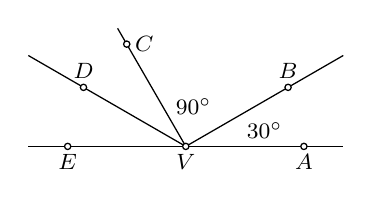
\begin{tikzpicture}
                % \clip (0,0) rectangle (14.000000,10.000000);
                {\footnotesize

                % Marking point V by circle
                \draw [line width=0.016cm] (4.000000,1.500000) circle (0.040000);%
                \draw (4.000000,1.500000) node [anchor=north] { $V$ };%

                % Marking point A by circle
                \draw [line width=0.016cm] (5.500000,1.500000) circle (0.040000);%
                \draw (5.500000,1.500000) node [anchor=north] { $A$ };%

                % Marking point E by circle
                \draw [line width=0.016cm] (2.500000,1.500000) circle (0.040000);%
                \draw (2.500000,1.500000) node [anchor=north] { $E$ };%

                % Drawing line A E
                \draw [line width=0.016cm] (2.000000,1.500000) -- (2.460000,1.500000);%
                \draw [line width=0.016cm] (2.540000,1.500000) -- (3.960000,1.500000);%
                \draw [line width=0.016cm] (4.040000,1.500000) -- (5.460000,1.500000);%
                \draw [line width=0.016cm] (5.540000,1.500000) -- (6.000000,1.500000);%

                % Marking point B by circle
                \draw [line width=0.016cm] (5.299038,2.250000) circle (0.040000);%
                \draw (5.299038,2.250000) node [anchor=south] { $B$ };%

                % Marking point C by circle
                \draw [line width=0.016cm] (3.250000,2.799038) circle (0.040000);%
                \draw (3.250000,2.799038) node [anchor=west] { $C$ };%

                % Marking point D by circle
                \draw [line width=0.016cm] (2.700962,2.250000) circle (0.040000);%
                \draw (2.700962,2.250000) node [anchor=south] { $D$ };%

                % Drawing line V D
                % \draw [line width=0.016cm] (4.519615,1.200000) -- (4.034641,1.480000);%
                \draw [line width=0.016cm] (3.965359,1.520000) -- (2.735603,2.230000);%
                \draw [line width=0.016cm] (2.666321,2.270000) -- (2.000000,2.654701);%

                % Drawing line V C
                % \draw [line width=0.016cm] (4.173205,1.200000) -- (4.020000,1.465359);%
                \draw [line width=0.016cm] (3.980000,1.534641) -- (3.270000,2.764397);%
                \draw [line width=0.016cm] (3.230000,2.833679) -- (3.133975,3.000000);%

                % Drawing line V B
                % \draw [line width=0.016cm] (3.480385,1.200000) -- (3.965359,1.480000);%
                \draw [line width=0.016cm] (4.034641,1.520000) -- (5.264397,2.230000);%
                \draw [line width=0.016cm] (5.333679,2.270000) -- (6.000000,2.654700);%

                % Marking point {30^\circ}
                \draw (5.000000,1.500000) node [anchor=south] { ${30^\circ}$ };%

                % Marking point {90^\circ}
                \draw (4.100000,1.800000) node [anchor=south] { ${90^\circ}$ };%
                }
            \end{tikzpicture}

        \end{figure}
    \end{naloga}






\newpage
%%%%%%%%%%%%%%%%%%%%%%%%%%%%%%%%%%%%%%%


\section{Vzporednost in pravokotnost}